\section{Organisation}
\subsection{Les outils utilisés}

Afin de nous coordonner et de gérer les versions, nous avons utilisé git. Le dépôt est accessible à l'adresse \url{https://github.com/Neressea/MovieManager}. \\
Pour générer l'UML et simplifier le lancement des tests unitaires, nous avons utilisé l'IDE Eclipse. \\
Nous pouvons aussi noter l'utilisation de jar externes pour le JDatePicker qui sert à la sélection de la date et pour les tests unitaires.

\subsection{UML du modèle}

L'UML du modèle a été généré à l'aide du module ObjectAid UML d'Eclipse. \\

\begin{figure}[!ht]
    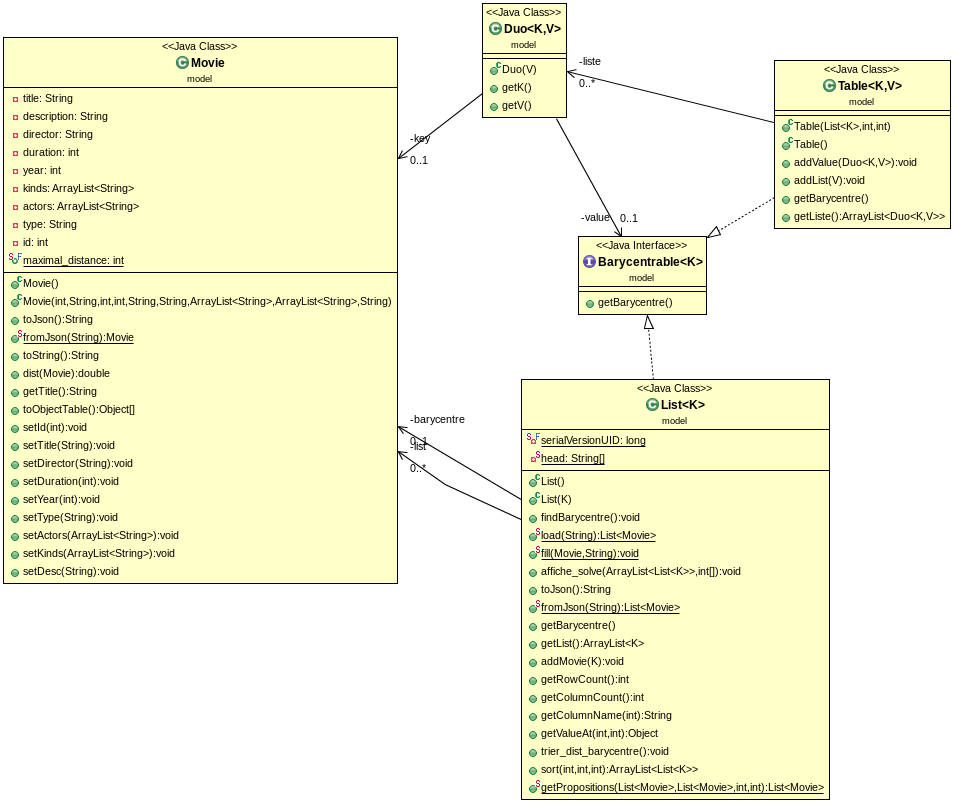
\includegraphics[width=1\textwidth]{./images/uml.png}
    \caption{UML du projet}
\end{figure}

Nous avons décidé de nous appuyer sur une structure en tables de hachage pour faciliter l'accès aux données lors des parcours et pour regrouper au préalable les films les plus similaires. \\
Les clés sont des films dits "barycentres" qui sont les plus représentatifs de leur groupe (c'est-à-dire que ce sont les films dont la distance globale à tous les autres est la plus faible). Les valeurs sont des listes de films ordonnées par rapport au film barycentre grâce au tri par sélection vu en TOP. \\
Le découpage en listes se fait grâce à une variante de l'algorithme des H-Means vu en mathématiques numériques. \\
Pour permettre une réalisation ultérieure du code, nous avons utilisé des types génériques pour laisser le programmeur libre de son implémentation. \\
On peut remarquer que l'on a créé une interface Barycentrable qui nous permet de limiter l'utilisation de Duo aux objets avec l'héritage.
Grâce à cela, nous pouvons appeler la méthode getBarycentre() à tout instant. \\

\subsubsection{Les raisons du modèle}

Nous avons préféré cette structure en table de hachage aux autres, notamment aux listes qui ne nous ont pas paru adaptée à la situation, autant pour les parcours lors de la recherche que pour les algorithmes de classification. \\
Nous l'avons aussi préférée à des structure en forme de graphe, car les temps de calcul et de recherche sont plus longs et elle n'est pas adaptée à un algorithme de partitionnement. \\
Les arbres auraient pu être intéressants pour la vitesse du traitement des données, mais il aurait été difficile au vu du temps imparti d'adapter des algorithmes de partitionnement aux arbres. 
